% Chapter 04
\chapter{An investigation into the relationship between cardiopulmonary exercise testing and body composition in patients undergoing major pancreatic surgery.}
\label{ch_bodycomp}

\lhead{Chapter \ref{ch_bodycomp}. \emph{CPET and Body Composition}} % This is for the header on each page - perhaps a shortened title

\clearpage
%----------------------------------------------------------------------------------------
\todo{Consider including relationship with systemic inflammation} 

zotero - richards-relationships-2012

\section{Introduction}
Major abdominal surgery especially for pancreatic disease is associated with significant morbidity and mortality. Patient selection is as important as identifying surgical treatable pathology in ensuring optimal outcomes. \parencite{balthazar_acute_2002}

\subsection{Role of preoperative CPET}
The role of cardiopulmonary exercise testing in the preoperative evaluation and risk assessment/stratification of patients undergoing major thoracic and abdominal surgery has become well established. A number of studies have shown that poor aerobic fitness demonstrated by a low $\dot{V}_{O_2}$AT or low $\dot{V}_{O_2}$Peak or both as measured at cardiopulmonary exercise testing is associated with increased morbidity and mortality after major surgery including bariartic\parencite{mccullough_cardiorespiratory_2006}, pancreatic\parencite{chandrabalan_pre-operative_2013,ausania_effects_2012}, liver \parencite{epstein_aerobic_2004}, cardiothoracic\parencite{brunelli_risk_2010, campione_oxygen_2010,torchio_exercise_2010} and abdominal aortic aneurysm surgery.\parencite{carlisle_mid-term_2007,thompson_cardiopulmonary_2011} CPET is now routinely used as part of the preoperative processes used to select patients for surgery as well as to help in decision making regarding preoperative care including the need for additional tests, preoperative and intraoperative optimisation, admission to critical care and postoperative care.
Patients are sometimes denied surgery if their performance at cardiopulmonary exercise testing is felt to be poor based on currently available evidence.

\subsection{The pathophysiological basis of CPET}
Aerobic fitness, as defined by the ability to perform physical exercise, is dependant on and often limited by the ability of the cardiorespiratory and circulatory systems (henceforth simply the cardiorespiratory system) to supply O2 to skeletal muscles at times of increased demand as well as remove the main end product of aerobic metabolism, namely CO2. Several factors play an important role in this increased response of the cardiorespiratory system. The most important factor is an increase in cardiac output which in healthy adults can increase by upto six-fold during exercise. Aside from increased stroke volume and heart rate, the redistribution of blood volume from the splanchnic circulation increases venous return to the heart. A consequent increase in pulmonary blood flow and skeletal blood flow occurs which in turn is assisted by vasodilation in these circulatory beds.

Oxygenation of the increased pulmonary blood flow and removal of the excess CO2 generated by aerobic exercise is effected by increased minute ventilation as a result of increase in its constituent factors namely respiratory rate and tidal volume. Oxygenation of skeletal muscle is further dependant on numerous other factors including the oxygen carrying capacity of blood (primary determinant being haemoglobin), adequate peripheral circulation and the ability of the mitochondria within the skeletal muscle to utilise the oxygen that is being delivered to them. 

It is clear that limitations in the patient's physiology resulting in inadequate or inappropriate response in any of the above mentioned factors will result in overall limitation of their aerobic fitness. Cardiopulmonary exercise testing allows the accurate measurement of most of these factors either directly or indirectly during dynamic exercise thus allowing identifying not only limitations in aerobic fitness but also the cause for such limitation. 

\subsection{Factors influencing aerobic fitness}
A low $\dot{V}_{O_2}$ has universally been attributed to low aerobic fitness due to an inadequate response of the cardiovascular and respiratory systems to increased oxygen demand during exercise. This is often thought to be due to cardiorespiratory disease, overt or sub-clinical. Occasionally, other factors such as anaemia, peripheral vascular disease and rarely, mitochondrial diseases have been recognised as factors contributing to low $\dot{V}_{O_2}$ or abnormalities in other parameters measured at cardiopulmonary exercise testing but these causes are less common in patients undergoing major abdominal surgery.

The most common parameters used to quantify perioperative risk in surgical patients are oxygen consumption at the anaerobic threshold ($\dot{V}_{O_2}$AT) and at peak exercise capacity ($\dot{V}_{O_2}$Peak). Conventionally these have been reported as per weight ratios (ml/kg/min) to allow comparison between patients. However, numerous studies on cardiorespiratory exercise physiology have reported that normalising $\dot{V}_{O_2}$ using total body weight leads to spurious correlation errors unfairly penalising obese subjects.\parencite{seltzer_body_1940, tanner_fallacy_1949, toth_examination_1993, batterham_modeling_1999, goran_total_2000, krachler_cardiopulmonary_2014} 

\subsection{Aims}
In chapter \ref{ch_cpet_outcomes}, we reported that low $\dot{V}_{O_2}$AT in patients undergoing pancreaticoduodenectomy was associated with increased incidence of postoperative pancreatic fistula and prolonged hospital stay. We also reported that patients with a $\dot{V}_{O_2}$AT less than 10 ml/kg/min were less likely to receive postoperative adjuvant chemotherapy as a result of postoperative complications, prolonged hospital stay and possibly due to lack of physiological reserve after surgery. However, we also observed that high BMI was associated with a low $\dot{V}_{O_2}$AT independent of all other clinicopathological characteristics. Moreover, most of our patients did not have overt cardiac or respiratory comorbidity to explain the very low levels of $\dot{V}_{O_2}$AT.

The aim of the present study was to explore the association between body composition, total body weight and the physiological parameters measured at cardiopulmonary exercise testing.

\clearpage
\section{Methods}

\subsection{Patients}
Patients scheduled to undergo pancreaticoduodenectomy for malignant or benign disease involving the head of the pancreas and periampullary region between August 2008 and October 2010 were included in this study. All data were recorded in a prospectively maintained database. Data was collected on demographics, preoperative clinicopathological characteristics including blood tests, body mass index, weight, height and the underlying surgical pathology. Detailed breath-by-breath data on a variety of physiological and gas-exchange parameters measured at cardiopulmonary exercise testing were also collected from a prospectively maintained database. Cardiopulmonary exercise testing methodolgy is discussed in Section \ref{sec:cpx_method} (p\pageref{sec:cpx_parameters})and a description of the parameters measured at cardiopulmonary exercise testing is provided in Section \ref{sec:cpx_parameters} (p\pageref{sec:cpx_parameters}).

\subsection{Calculation of body composition}
Computed tomography of the abdomen, performed as part of the routine preoperative staging, was used to calculate body composition based on previously published and well established methods.\parencite{bredella_comparison_2010,shen_total_2004}

%http://regionstraumapro.com/post/16349545265 - Excellent description of CT window width(W) and level/center(C)
The coronal and sagittal reconstructions were used to accurately identify the L3 and L4 vertebrae. The CT window width (W) was set at 400 and the level/center (C) was set at 40. This allowed tissue between -160 HU and +240 HU to be represented in grayscale with adequate contrast between tissues of interest. The cross-sectional images at these levels where then exported as gray-scale bitmap images. The scale in millimeters was included with every image. A representative image is shown in Fig. 1.The GNU Image Manipulation Program (GIMP), an advanced, free, open-source, raster graphics editor was used for analysis of all images (www.gimp.org). The use of GIMP to analyse cross-sectional imaging for body composition has been described previously although by using a different technique to what has been employed by us. \parencite{anblagan_measurement_2013}

The first step involved converting the bitmap images into JPEG images using lossy compression set at 85\% to minimise sharp transitions between grey areas of very similar colour values. This allowed more consistent selection of contiguous areas of similar grey shades. 

The next step involved standardising the scale of all images by dividing the length of the scale on every image by the number of pixels along the scale thus providing a length in millimetres for each pixel in each image. As pixels on a CT image are square, the area of each pixel was calculated as a square of its length. 

The Fuzzy Select (Magic Wand) tool was used to select contiguous areas of similar colour while simultaneously using visual confirmation that the correct anatomical structures had been selected without overspill into unwanted areas. The number of pixels within the selection was obtained using the 'Histogram' dialog window and entered into an excel spreadsheet against the selected area of interest. The area in mm2 was calculated by multiplying the number of pixels by the area of each pixel.

\textbf{Selecting tissue compartments}:

The sequence of steps followed to calculate the area of each tissue compartment is depicted in Fig. \ref{fig:bc_ct_gimp} on p	\pageref{fig:bc_ct_gimp}. The total cross-sectional area of the abdomen at the level of L3/L4 was calculated by first selecting all the empty space outside the image followed by inverting this selection. This is depicted in Fig. \ref{fig:bc_ct_csa}. Subcutaneous fat in the image was selected using the Fuzzy Select tool (if necessary by choosing multiple times and removing any unnecessary areas) as depicted in Fig. \ref{fig:bc_ct_sat}. The same process was repeated for visceral adipose tissue and skeletal muscle as depicted in Fig. \ref{fig:bc_ct_vat} and Fig. \ref{fig:bc_ct_sm} respectively. Every selection was visually confirmed for anatomical accuracy by using the layer selection tool to inspect the area under selection as shown in the insets in each of the images.
%CT slices images x 4
\begin{figure}[htbp]
	\centering
	\begin{subfigure}{0.45\textwidth}
		\centering
		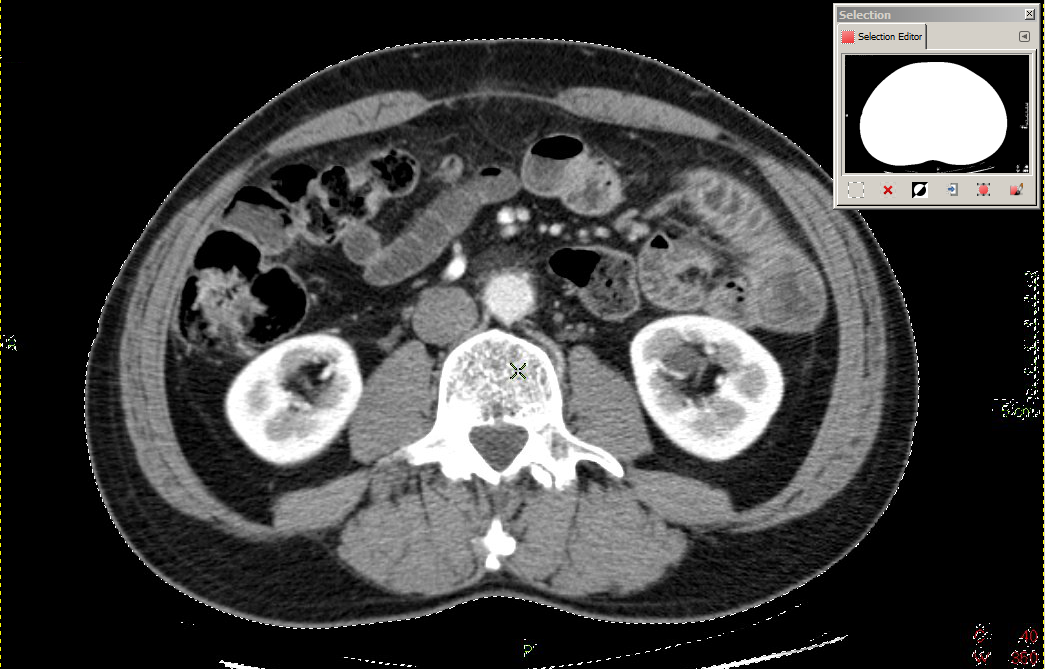
\includegraphics[width=\textwidth]{Figures/bc_ct_csa}
		\caption{Total Cross-sectional Area}
		\label{fig:bc_ct_csa}
	\end{subfigure}
	\begin{subfigure}{0.45\textwidth}
		\centering
		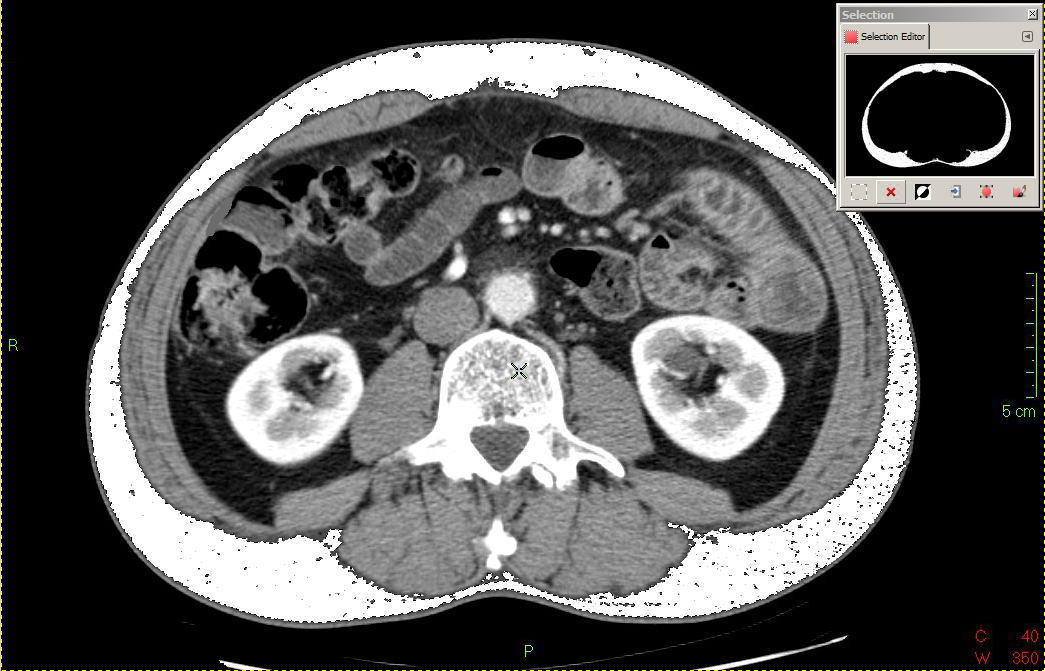
\includegraphics[width=\textwidth]{Figures/bc_ct_sat}
		\caption{Subcutaneous Adipose Tissue$^*$}
		\label{fig:bc_ct_sat}
	\end{subfigure}
	\hfill
	\begin{subfigure}{0.45\textwidth}
		\centering
		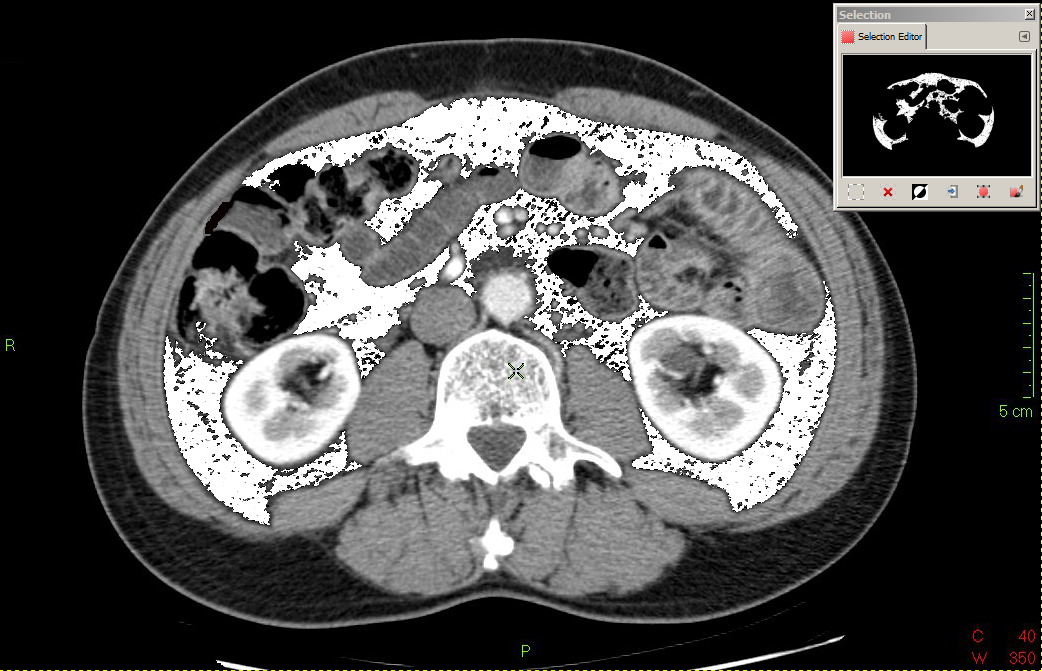
\includegraphics[width=\textwidth]{Figures/bc_ct_vat}
		\caption{Visceral Adipose Tissue$^*$}
		\label{fig:bc_ct_vat}
	\end{subfigure}
	\begin{subfigure}{0.45\textwidth}
		\centering
		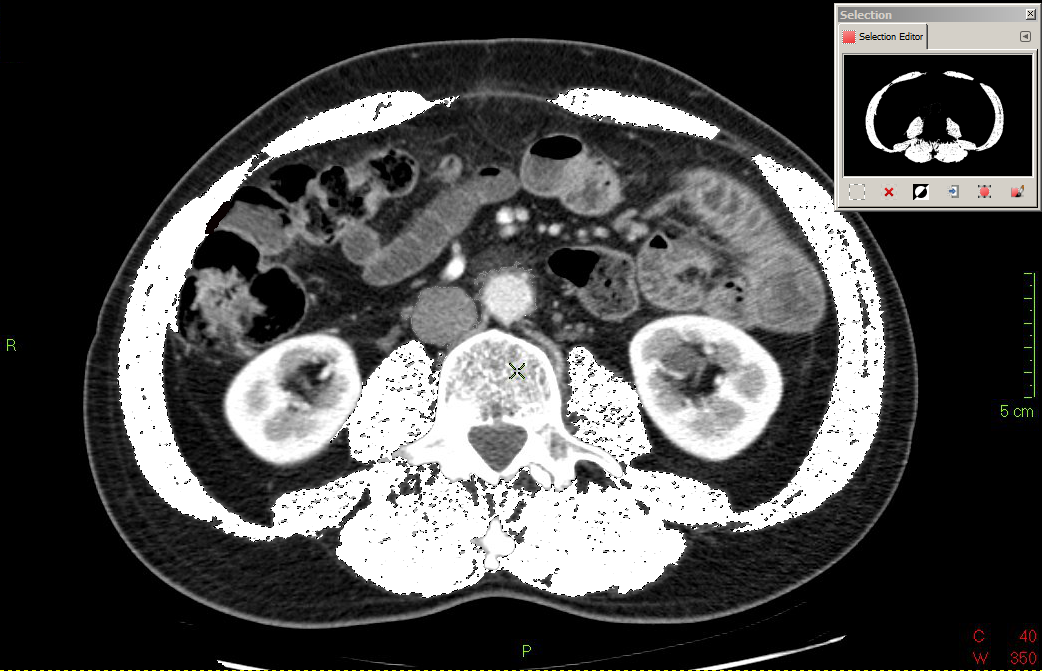
\includegraphics[width=\textwidth]{Figures/bc_ct_sm}
		\caption{Skeletal Muscle$^*$}
		\label{fig:bc_ct_sm}
	\end{subfigure}
	
	\caption{Selection of components of body composition from CT images using GIMP.}($^*$ The selected area has been removed for representation purposes. The inset confirms the area selected.)
	\label{fig:bc_ct_gimp}
	
\end{figure}

\subsection{Cardiopulmonary exercise testing}
All patients performed cardiopulmonary exercise testing on a cycle ergometer as described in Section \ref{sec:cpx_method}. Raw data of all breath-by-breath parameters averaged every 10 seconds was collected for analysis. The first three minutes of the recorded data were during the rest period when the patients were on the exercise bike but did not exercise. The average of each parameter measured between the first and second minute (6 readings) was treated as the rest value. Anaerobic threshold was identified using previously established methods and all corresponding parameters at this point were recorded.\parencite{beaver_new_1986,sue_metabolic_1988} Peak exercise was identified by the maximum oxygen consumption recorded towards the end of the exercise period and all other parameters recorded at this point were considered as peak exercise values. 

\subsection{Statistics}

All analyses were performed using the SPSS statistical package for Microsoft Windows (version 22 ). Comparison between body composition and cardiopulmonary exercise testing parameters was done using Partial correlations controlling for the effect of gender (and/or age). All p-values reported are two-sided. The relationship between body composition and preoperative clinico-pathological characteristics (as categorical variables) was analysed using the Mann-Whitney U test for variables with two categories or the Kruskal-Wallis test for variables with more than two categories. Previously established cut-offs were used for categorising continuous variables where applicable. The level of significance was set at $p<0.05$.

\clearpage
\section{Results}

\subsection{Body composition and Clinico-pathological characteristics}
Eighty-two patients (35 male) were included in the study. The clinico-pathological characteristics of the study patients and their relationship to body composition is shown in Table \ref{table:bc_clinical} on page \pageref{table:bc_clinical}. There were several significant associations between clinico-pathological variables and body composition as depicted in this table.

	%Table 1
\begin{sidewaystable}[p]
\caption{The relationship between body composition and clinico-pathological characteristics of patients undergoing major pancreatic surgery.}
\label{table:bc_clinical}
\centering
\begin{tabular}{l c c | c c c | c c c | c c c}
	           &           &    & CSA   &       &          & TAT   &       &          & SM    &      &  \\
	           &           & n  & Mean  & SD    & p        & Mean  & SD    & p        & Mean  & SD   & p        \\ \hline
	Age        & $<$ 65    & 35 & 688.6 & 192.8 & 0.386    & 297.0 & 178.5 & 0.309    & 128.7 & 29.4 & 0.590    \\
	           & $\geq$ 65 & 47 & 704.3 & 150.6 &          & 322.7 & 156.6 &          & 124.1 & 31.3 &  \\
	Gender     & M         & 52 & 738.4 & 171.2 & $<$0.001 & 316.6 & 170.8 & 0.665    & 141.3 & 26.1 & $<$0.001 \\
	           & F         & 30 & 626.9 & 141.6 &          & 303.0 & 159.3 &          & 99.7  & 15.6 &  \\
	BMI        & $\leq$ 25 & 39 & 579.9 & 103.6 & $<$0.001 & 205.9 & 97.0  & $<$0.001 & 114.6 & 26.6 & 0.002    \\
	           & 25-30     & 31 & 754.0 & 109.4 &          & 350.6 & 99.6  &          & 136.0 & 30.4 &  \\
	           & $>$ 30    & 12 & 934.6 & 145.4 &          & 554.6 & 185.9 &          & 137.6 & 30.9 &  \\
	SMID       & $>$ 3     & 49 & 684.4 & 163.1 & 0.366    & 288.7 & 175.5 & 0.040    & 123.2 & 31.6 & 0.380    \\
	           & $\leq$ 3  & 21 & 718.5 & 187.2 &          & 365.7 & 165.0 &          & 128.2 & 31.9 &  \\
	Pathology  & Benign    & 10 & 737.9 & 228.4 & 0.766    & 352.8 & 278.1 & 0.955    & 122.4 & 24.0 & 0.788    \\
	           & Malignant & 72 & 692.0 & 160.3 &          & 305.9 & 145.9 &          & 126.6 & 31.3 &  \\
	VO$_2$AT   & $\geq$ 10 & 39 & 659.8 & 173.1 & 0.035    & 257.2 & 144.3 & 0.003    & 131.5 & 33.2 & 0.111    \\
	           & $<$ 10    & 43 & 731.9 & 159.4 &          & 361.0 & 170.1 &          & 121.2 & 27.1 &  \\
	VO$_2$Peak & $\geq$ 16 & 35 & 663.8 & 172.5 & 0.112    & 249.3 & 143.0 & 0.002    & 136.9 & 31.1 & $<$0.001 \\
	           & $<$ 16    & 47 & 722.8 & 163.6 &          & 358.1 & 167.7 &          & 118.0 & 27.5 &  \\
	CRP        & $\leq$ 10 & 50 & 691.4 & 183.1 & 0.512    & 303.7 & 145.2 & 0.985    & 128.7 & 33.5 & 0.392    \\
	           & $>$ 10    & 32 & 707.3 & 146.4 &          & 324.0 & 195.6 &          & 122.0 & 24.7 &  \\
	Albumin    & $\geq$ 35 & 32 & 743.8 & 173.5 & 0.062    & 339.4 & 179.3 & 0.213    & 134.5 & 34.1 & 0.054    \\
	           & $<$ 35    & 50 & 668.1 & 160.8 &          & 293.8 & 155.8 &          & 120.7 & 26.7 &  \\
	Hb         & $\geq$ 12 & 50 & 698.0 & 172.4 & 0.725    & 292.5 & 145.4 & 0.372    & 133.4 & 32.1 & 0.005    \\
	           & $<$ 12    & 32 & 697.1 & 166.2 &          & 341.5 & 192.2 &          & 114.6 & 23.6 &  \\
	PPS        & $\leq$ 14 & 41 & 708.7 & 169.8 & 0.444    & 323.2 & 155.0 & 0.347    & 129.8 & 34.5 & 0.351    \\
	           & $>$ 14    & 41 & 686.5 & 169.5 &          & 300.0 & 177.1 &          & 122.4 & 25.5 &  \\
	Cardiac    & No        & 43 & 675.2 & 185.7 & 0.109    & 305.5 & 195.5 & 0.208    & 120.7 & 33.0 & 0.047    \\
	disease    & Yes       & 39 & 722.3 & 146.8 &          & 318.4 & 127.6 &          & 132.0 & 26.4 &  \\
	Resp.      & No        & 72 & 704.8 & 170.8 & 0.269    & 319.0 & 169.3 & 0.342    & 125.8 & 30.5 & 0.810    \\
	disease    & Yes       & 10 & 646.1 & 153.2 &          & 258.3 & 133.3 &          & 128.0 & 30.9 &
\end{tabular}
\end{sidewaystable}

\subsection{Body Composition in Normal BMI vs Overweight/Obese Patients}
The body composition differences between patients with a normal BMI and patients who are overweight or obese is shown in Figure \ref{fig:bc_gender_bmi} on page \pageref{fig:bc_gender_bmi}. There were significant differences in the proportion of subcutaneous adipose tissue versus visceral adipose tissue between males and females. Men had generally larger cross-sectional area, less SAT but greater VAT and SM areas. However, the proportion of skeletal muscle in both males and females decreased significantly with increasing BMI.

\begin{figure}[h]
	\centering
	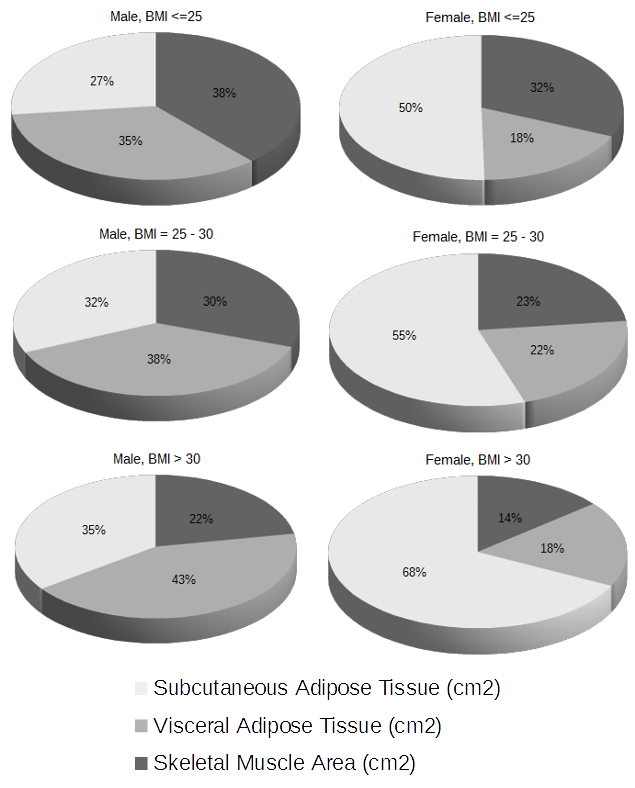
\includegraphics[width=0.8\textwidth]{Figures/bc_gender_bmi_pie}
	\caption{Differences in body composition according to gender and body mass index.}
	\label{fig:bc_gender_bmi}
\end{figure}

The proportion of skeletal muscle area at L3/L4 decreases from 38\% in male patients with normal BMI to 22\% in males who are obese. There was a greater decrease in the proportion of skeletal muscle area in females with normal BMI (32\%) and obese females (14\%). The higher weight in the high BMI patients was due to a disproportionate increase in adipose tissue rather than skeletal muscle. Moreover, the distribution of the adipose tissue differed between males and females with visceral adipose tissue contributing more to weight in obese males (43\% VAT vs. 35\% SAT) while obese females had a greater proportion of subcutaneous adipose tissue than visceral adipose tissue (68\% SAT vs. 18\% VAT)

\subsection{Correlation with Pulmonary Function Tests}

Partial correlation analysis was performed to study the relationship between pulmonary function tests and body composition. It has been well-established in previous studies that pulmonary function tests are correlated with age and gender and the analysis was therefore adjusted for these two variables. Forced Vital Capacity (FVC, litres), Forced Expiratory Volume in 1 second (FEV1, litres) and the ratio FEV1/FVC (Tiffeneau-Pinelli index,\%) were compared against the various components of body composition. Both FVC and FEV1 were positively correlated with skeletal muscle area but not with adipose tissue area or total cross-sectional area. FEV1/FVC was not correlated with any of the body composition components. This would indicate that pulmonary function was dependent on skeletal muscle area while FEV1/FVC, a calculated index to quantify restrictive or obstructive lung disease, was not associated with skeletal muscle area. These results are shown in Table \ref{table:bc_cpet} on page \pageref{table:bc_cpet}.

\subsection{Correlation with Exercise Load}

%Table 2
\begin{table}[p]
	\caption{The relationship between body composition and cardiopulmonary exercise testing controlled for gender in patients undergoing major pancreatic surgery.}
	\label{table:bc_cpet}
	\centering
	\renewcommand{\arraystretch}{1.4} %Increases space between rows
	\setlength{\tabcolsep}{9pt} %sets the space between columns
	%\hline\noalign{\smallskip} %increases space after the line
	\begin{tabular}{|l | c c | c c | c c|}
		\hline
		                   & \multicolumn{2}{|c|}{CSA} & \multicolumn{2}{|c|}{TAT} & \multicolumn{2}{|c|}{SM}      \\
		Variable           & $\rho$ & p                & $\rho$ & p                & $\rho$ & p                    \\ \hline
		\multicolumn{7}{|c|}{Pulmonary Function Tests$^a$}                                                         \\ \hline
		FVC                & -0.026 & 0.823            & -0.112 & 0.325            & 0.303  & 0.007                \\
		FEV1               & 0.083  & 0.468            & -0.012 & 0.919            & 0.350  & 0.002                \\
		FEV1/FVC           & 0.096  & 0.398            & 0.101  & 0.374            & 0.003  & 978                  \\ \hline
		\multicolumn{7}{|c|}{At Rest$^b$}                                                                          \\ \hline
		Minute Ventilation & 0.104  & 0.358            & 0.116  & 0.307            & 0.136  & 0.230                \\
		Tidal Volume       & 0.234  & 0.037            & 0.116  & 0.305            & 0.301  & 0.007                \\
		Absolute VO2       & 0.251  & 0.025            & 0.164  & 0.145            & 0.353  & 0.001                \\
		Corrected VO2      & -0.473 & $<$0.001         & -0.482 & $<$0.001         & -0.194 & 0.085                \\
		O2 Pulse           & 0.303  & 0.006            & 0.141  & 0.212            & 0.192  & 0.087                \\ \hline
		\multicolumn{7}{|c|}{At Anaerobic Threshold$^b$}                                                           \\ \hline
		Exercise Load      & 0.173  & 0.123            & 0.105  & 0.349            & 0.377  & 0.001                \\
		Minute Ventilation & 0.203  & 0.069            & 0.198  & 0.076            & 0.263  & 0.018                \\
		Tidal Volume       & 0.259  & 0.020            & 0.170  & 0.128            & 0.436  & $<$0.001             \\
		Absolute VO2       & 0.340  & 0.002            & 0.231  & 0.038            & 0.463  & $<$0.001             \\
		Corrected VO2      & -0.373 & 0.001            & -0.400 & $<$0.001         & -0.078 & 0.487                \\
		O2 Pulse           & 0.432  & $<$0.001         & 0.242  & 0.029            & 0.338  & 0.002                \\ \hline
		\multicolumn{7}{|c|}{At Peak Exercise$^b$}                                                                 \\ \hline
		Exercise Load      & 0.113  & 0.314            & 0.020  & 0.859            & 0.373  & 0.001                \\
		Minute Ventilation & 0.139  & 0.217            & 0.112  & 0.321            & 0.242  & 0.029                \\
		Tidal Volume       & 0.239  & 0.032            & 0.138  & 0.219            & 0.409  & $<$0.001             \\
		Absolute VO2       & 0.192  & 0.086            & 0.093  & 0.407            & 0.375  & 0.001                \\
		Corrected VO2      & -0.334 & 0.002            & -0.374 & 0.001            & -0.027 & 0.813                \\
		O2 Pulse           & 0.377  & 0.001            & 0.261  & 0.019            & 0.363  & 0.001                \\ \hline
		\multicolumn{7}{l}{CSA - Cross-sectional area, TAT - Total Adipose Tissue area}                            \\
		\multicolumn{7}{l}{SM - Skeletal Muscle area, all in cm$^2$.}                                              \\
		\multicolumn{7}{l}{$\rho$ - Pearson's r adjusted for \textit{a} - age and sex and \textit{b} - sex.}
	\end{tabular}
\end{table}

Exercise loads achieved at anaerobic threshold and at peak exercise capacity (at volitional stop rather than maximal exercise) were plotted against skeletal muscle area and subcutaneous adipose tissue area measured at L3/L4 to create scatter-plots(Fig. \ref{fig:bc_load_vs_sm}, p\pageref{fig:bc_load_vs_sm}. Exercise load correlated positively with skeletal muscle area both at anaerobic threshold ($r^{2} = 0.284, p < 0.001$, Fig. \ref{fig:bc_at_load_vs_sm}) and at peak exercise ($r^{2} = 0.350, p < 0.001$, Fig. \ref{fig:bc_pk_load_vs_sm}). However, no correlation was identified between exercise loads achieved and subcutaneous adipose tissue area either at anaerobic threshold ($r^{2} = 0.004, p = 0.587$) or peak exercise ($r^{2} = 0.020, p = 0.206$). 

\begin{figure}[htb]
	\centering
	\begin{subfigure}[b]{0.45\textwidth}
		\centering
		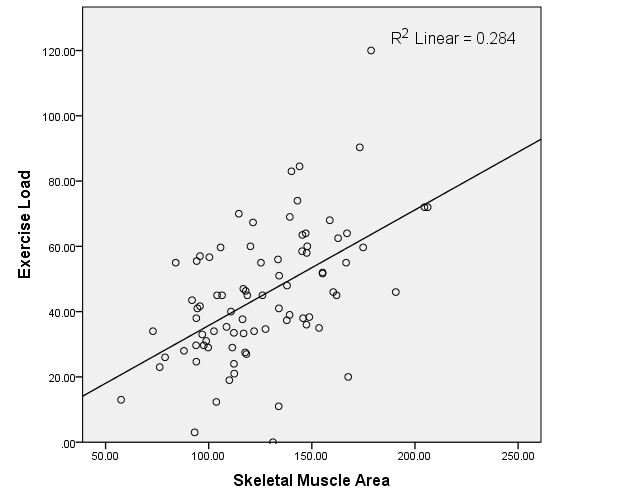
\includegraphics[width=\textwidth]{Figures/bc_scatter_atLoad_skeletal}
		\caption{Anaerobic Threshold}
		\label{fig:bc_at_load_vs_sm}
	\end{subfigure}
	\hfill
	\begin{subfigure}[b]{0.45\textwidth}
		\centering
		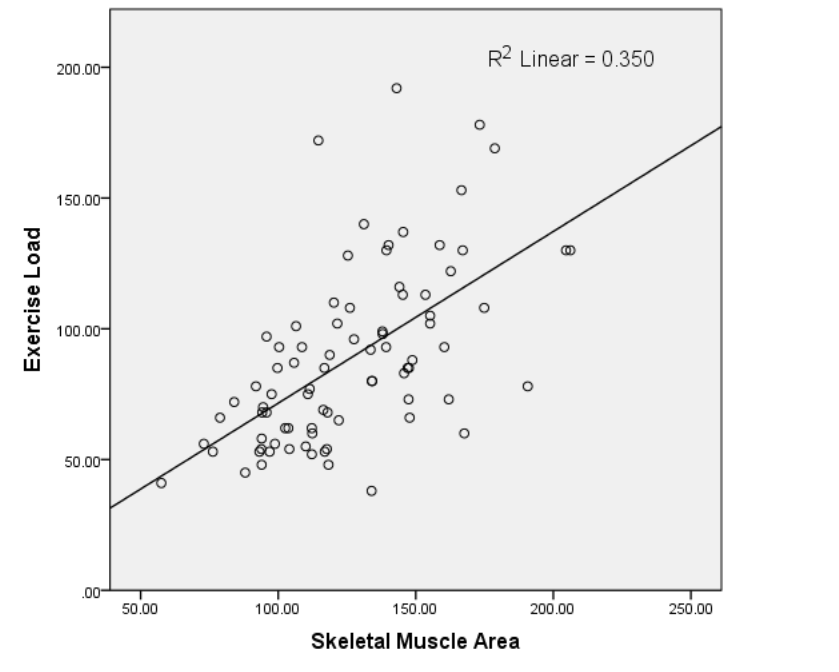
\includegraphics[width=\textwidth]{Figures/bc_scatter_pkLoad_skeletal}
		\caption{Peak Exercise}
		\label{fig:bc_pk_load_vs_sm}
	\end{subfigure}
	\caption{Correlation between exercise load and skeletal muscle area.}	
	\label{fig:bc_load_vs_sm}
		
\end{figure}

%This would suggest as one would expect that exercise capacity is mostly related to skeletal muscle volume rather than subcutaneous adipose tissue. - Move this to discussion 

\subsection{Correlation with Oxygen consumption}

The correlations between cardiopulmonary exercise parameters and body composition were adjusted for gender. Our own findings (\ref{ch_cpet_jaundice}) and the findings of other authors suggest that age is not related to $\dot{V}_{O_2}$AT or $\dot{V}_{O_2}$Peak and therefore no adjustments were made for age. The results of this analysis are shown in Table \ref{table:bc_cpet} (p\pageref{table:bc_cpet}).

% Absolute oxygen consumption at the anaerobic threshold in litres per minute was plotted against the total cross-sectional area, subcutaneous adipose tissue area, visceral adipose tissue area and skeletal muscle area. This was repeated by plotting the oxygen consumption at anaerobic threshold corrected for total body weight (in millilitres/kg/min) against the total cross-sectional area, subcutaneous adipose tissue area, visceral adipose tissue area and skeletal muscle area. These scatter-plots are shown in FigureX1. The same was repeated for oxygen consumption at peak exercise and at rest. 

Tidal volume ($\dot{V}_T$, litres) was significantly correlated with skeletal muscle area at all phases of exercise including at rest, anaerobic threshold and peak exercise. There was a statistically significant but weak positive correlation between minute ventilation ($\dot{V}_E$, litres) and skeletal muscle at anaerobic threshold and peak exercise but not at rest. There was no correlation between either of these measures of pulmonary function and total adipose tissue area at any phase of exercise.

%----------------------------------------------------------------------------------------------
% Correlation between body composition and $\dot{V}_{O_2}$AT before and after correction for total body weight.
\begin{figure}[htb]
	\centering
	\begin{subfigure}[b]{0.45\textwidth}
		\centering
		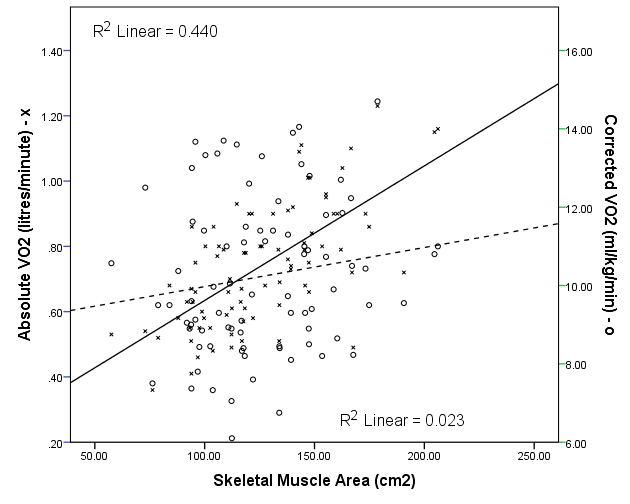
\includegraphics[width=\textwidth]{Figures/bc_scatter_VO2_skeletal}
		\caption{$\dot{V}_{O_2}$AT vs. Skeletal Muscle}
		\label{fig:bc_scatter_VO2_skeletal}
	\end{subfigure}
	\hfill
	\begin{subfigure}[b]{0.45\textwidth}
		\centering
		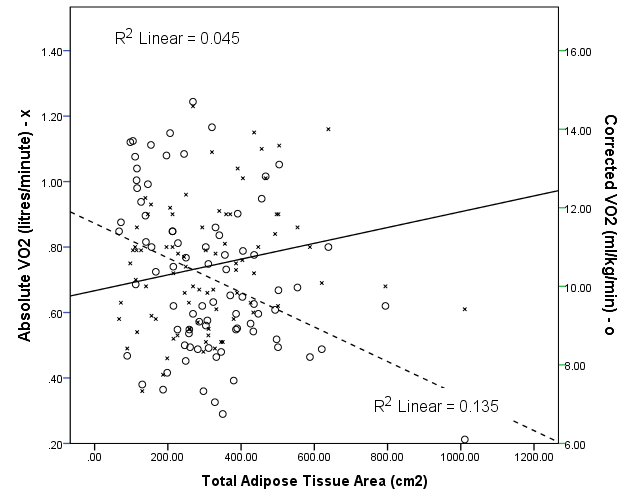
\includegraphics[width=\textwidth]{Figures/bc_scatter_VO2_TAT}
		\caption{$\dot{V}_{O_2}$AT vs. Total Adipose Tissue}
		\label{fig:bc_scatter_VO2_TAT}
	\end{subfigure}
	\caption{Correlation between body composition and $\dot{V}_{O_2}$AT before and after correction for total body weight.}	
	\label{fig:bc_scatter_VO2_bodycomp_reversal}
\end{figure}
%----------------------------------------------------------------------------------------------

Absolute $\dot{V}_{O_2}$ (litres/min) had a strong positive correlation with skeletal muscle area at rest ($\rho = 0.125, p = 0.001$), at anaerobic threshold ($\rho = 0.463, p<0.001$) and at peak exercise ($\rho = 0.375, p<0.001$). However, this correlation was lost after correction of $\dot{V}_{O_2}$ for total body weight and in fact there was a non-significant change in the direction of correlation to the negative.

Absolute $\dot{V}_{O_2}$ (litres/min) had no correlation with total adipose tissue at rest or at peak exercise and only a weak correlation at anaerobic threshold. However, when it was corrected for total body weight, there was a strong correlation between corrected $\dot{V}_{O_2}$ (mls/kg/min)and total adipose tissue at rest ($\rho = -0.482, p<0.001$), anaerobic threshold ($\rho = -0.400, p<0.001$) and peak exercise ($\rho = -0.374, p = 0.001$).

The loss of the physiological relationship between $\dot{V}_{O_2}$ and skeletal muscle after correcting for total body weight is shown in Fig.\ref{fig:bc_scatter_VO2_skeletal} and the creation of a spurious relationship with total adipose tissue after correction for total body weight is shown in Fig. \ref{fig:bc_scatter_VO2_TAT}.

%$\dot{V}_{O_2}$ corrected to height seems to correlate best with BC and everything else
\clearpage

\section{Discussion}

The results of this study show that the most important cardiopulmonary exercise test parameters as used for preoperative risk evaluation in surgery are influenced significantly by the patient's body composition. 

\subsection{Oxygen consumption and body composition}

The positive correlation between absolute $\dot{V}_{O_2}$ and skeletal muscle area is easily explained by the physiology of aerobic exercise. During periods of increased physical activity, the greater oxygen demand is primarily due to increased metabolic activity within the skeletal muscle. 

Current convention is to report $\dot{V}_{O_2}$ measured at cardiopulmonary exercise testing according the following formula: 
\[Corrected\ \dot{V}_{O_2} (mls.kg^{-1}.min^{-1}) = \frac{Absolute\ \dot{V}_{O_2}\ (litres.min^{-1}) * 1000}{Total\ body\ weight\ (kg)}\]

In a previous analysis (refer to chapter and table), we reported that there was a significant negative correlation between $\dot{V}_{O_2}$ at anaerobic threshold and the patient's body mass index in spite of no observable cardiopulmonary comorbid disease. 

The results of the present study suggest that the negative correlation between corrected $VO_{2}$ (mls/kg/min) and BMI is consequent to the reporting convention rather than due to any pathophysiological effect of obesity. 

The loss of the strong positive correlation between absolute $VO_{2}$ (litres/min) and skeletal muscle area after correcting for body weight further supports the argument that the corrected value under-reports aerobic capacity in obese patients. Moreover, the lack of correlation between pulmonary function tests, tidal volume and minute ventilation and adipose tissue area as well as the slight but statistically significant positive correlation between O2Pulse and adipose tissue area appear to suggest that adiposity did not contribute to poor cardiopulmonary exercise performance in this cohort of patients.

\subsection{Comparison with previous studies}
Our findings are similar to those reported by several authors previously. The relationship between body size, body composition and aerobic capacity both at rest and during exercise has been studied extensively for over a hundred years. 

Seltzer reported in his 1940 study of 34 subjects, that the individuals who were more "lateral" than "linear" had lower oxygen intakes per kilo body weight.\parencite{seltzer_body_1940} Tanner in his article titled \textit{"Fallacy of per-weight and per-surface area standards, and their relation to spurious correlation"}\parencite{tanner_fallacy_1949} in the Journal of Applied Physiology in 1947 recognised the dangers of expressing physiological variables as a function of total body mass. In a detailed anaysis comparing $\dot{V}_{O_2}$ and body build, he concludes that \textit{"as the index wt./stature increases, O2/wt. must be expected to decrease purely as a result of the method used for representing the data." }

Batterham et al studied 1314 apparently healthy men employed at the National Aeronautics and Space Administration Johnson Space Center in Houston, Texas.\parencite{batterham_modeling_1999} The authors report that as body mass increased, the proportion composed of fat-free mass decreased. They also found that fat-free mass had a linear relationship with oxygen consumption while total body mass did not. They suggest that ideally estimates of fat-free mass should be used in the representation of oxygen consumption to allow more reliable comparison between subjects. 

Janz et al studied oxygen consumption and aerobic capacity in adolescents over several years as part of the Muscatine study and reported their findings in 1997\parencite{janz_three-year_1997} and 1998.\parencite{janz_longitudinal_1998} Aerobic capacity in the form of $\dot{V}_{O_2}$peak was evaluated annually in 126 children (mean age 10.3 years) for five years. Body composition changes were also tracked over this period. They reported on the changes in body composition that occur over time and the differences in these changes between circum-pubertal boys and girls. They reported on the significant difficulties in normalising $\dot{V}_{O_2}$ using total body mass and suggested that fat-free mass was the most appropriate variable for normalising $\dot{V}_{O_2}$. They found that $\dot{V}_{O_2}$ normalised using total body mass underestimated aerobic fitness levels of heavier boys and girls. However, this underestimation was greater in girls than in boys. 

Goran et al reported that total body fat did not affect maximal aerobic capacity.\parencite{goran_total_2000} They reported on $\dot{V}_{O_2}$max in obese women before and after weight loss. $\dot{V}_{O_2}$max corrected for total body weight was significantly lower in the obese state while $\dot{V}_{O_2}$max corrected for fat-free mass did not change significantly after weight loss. They also reported that the limiting factor in the obese state was not the cardio-respiratory system but the fact that it was more difficult for obese individuals to do the same amount of work as a normal weight person in weight-bearing activities. This is likely due to the extra fat mass in these individuals that did not contribute to aerobic capacity but instead may increase the exercise load.

These findings have been replicated by several other authors in different subject groups.\parencite{loftin_scaling_2001,  lemaitre_maximum_2006,savonen_current_2012, krachler_cardiopulmonary_2014} Several of the above studies also recommend using allometric scaling to avoid the confounding effects of total body weight. However, this has not gained widespread clinical use.

In a study aimed at determining the optimal method of expressing $\dot{V}_{O_2}$max, Maciejczyk and coworkers analysed the differing influence of body fat and lean body mass on aerobic performance in a two groups of physically fit men categorised based on their body fat percentage.\parencite{maciejczyk_influence_2014} They reported that high body mass regardless of composition was correlated negatively with $\dot{V}_{O_2}$ when it was corrected for total body weight penalising otherwise fit men purely based on the proportion of body weight that was contributed by body fat. However, when $\dot{V}_{O_2}$ was corrected for lean body mass, they found that the results were similar between the low body fat and high fat body groups. They, similar to Goran et al\parencite{goran_total_2000}, recommend that $\dot{V}_{O_2}$ be normalised to lean body mass rather than total body weight.

The conclusion from the above studies would be that oxygen consumption normalised for total body weight unfairly penalises obese patients in the absence of true impairment of cardio-respiratory function. This has significant clinical implications as outlined below.

\subsection{Clinical implications of spurious correlation}
Older et al in their pioneering study in 1993 reported that $\dot{V}_{O_2}$AT < 11mls/kg/min was associated with increased mortality in elderly patients undergoing major abdominal surgery.\parencite{older_preoperative_1993} While they did not provide any data on other preoperative or intra-operative factors, they concluded that cardiopulmonary exercise testing was useful in predicting postoperative outcome. However, this first report on the use of cardiopulmonary exercise testing as a preoperative risk assessment tools repeatedly states that a $\dot{V}_{O_2}$AT < 11mls/kg/min represented cardiac failure. This association is repeated in their later work on 548 patients which also showed a clear association between $\dot{V}_{O_2}$AT < 11mls/kg/min and mortality due to cardiovascular causes. \parencite{older_cardiopulmonary_1999} The concepts of \textit{'surgical anaerobic threshold'} and \textit{'postoperative cardiac failure'} were introduced later and were described as the \textit{'inability of the heart to meet the demand of postoperative stress.'}\parencite{society_ats/accp_2003}

Swart and Carlisle reported that $\dot{V}_{O_2}$AT < 11mls/kg/min in patients undergoing open colorectal surgery was associated with adverse outcomes.\parencite{swart_case-controlled_2012} However, the proportion of females in the low $\dot{V}_{O_2}$AT group was significantly greater than that in the normal $\dot{V}_{O_2}$AT groups (24\% vs 51\%). The average $\dot{V}_{O_2}$AT in men calculated from the data presented in their paper was 11.02 mls/kg/min while in women it was 9.81 mls/kg/min. In a study by Wilson et al that reported cardiopulmonary exercise testing predicted outcome in major elective intra-abdominal surgery, the proportion of females in the low $\dot{V}_{O_2}$AT group was 51\% while it was 28\% in the group with normal AT.\parencite{wilson_impaired_2010} There was no data presented on body mass index in this study.

This is similar to the findings in our cohort of patients. This may have been due to the increased incidence of obesity especially in the subcutaneous plane as we have found in our cohort of patients as shown in Fig. \ref{fig:bc_figure1}.

It is clear from the review presented in Chapter 1, that cardiopulmonary exercise testing is useful in predicting risk after major surgery. Cardiopulmonary exercise testing has become ubiquitous in the preoperative workup of complex surgical patients. However, the results of the present study suggest that the results especially in the obese, female patient must be interpreted with caution, especially when used to select patients who may be declined surgery based on their cardiopulmonary exercise test results.

\subsection{Measuring impact of Prehabilitation}

Where time to surgery is not critical, prehabilitation has gained an increasingly important role in optimising patients for surgery and mitigating the effects of neoadjuvant oncological therapy. Cardiopulmonary exercise testing has been reported to be a useful objective measure of the impact of prehabilitation in surgical patients.\parencite{west_effect_2015}

The design of such prehabilitation programs must not depend solely on body weight adjusted parameters of cardiopulmonary exercise testing when assessing the success of the interventions in these programs. Instead, improvement in the absolute values of $\dot{V}_{O_2}$AT and $\dot{V}_{O_2}$Peak in conjunction with other parameters that are not affected by body composition such as O2Pulse, tidal volume\parencite{jones_effects_2007} or maximal exercise load may provide more reliable evidence of improvement in aerobic capacity.

%This needs to be expanded significantly. 

%Mention studies that have used VE/VCO2. 
%I think there is a study in bariatrics where bmi and at were independent predictors. 
%Mention studies that used predicted VO2 or absolute $\dot{V}_{O_2}$ where calculated AT was not useful. 
%This should give me at least another 2 paragraphs













